\documentclass{article}
\usepackage[dvipsnames]{xcolor}
\usepackage[paperwidth=10cm, paperheight=6cm, margin = 0cm, top=0.5cm]{geometry}
\usepackage{amsmath}



\usepackage{pgf}
\usepackage{tikz}
\usetikzlibrary{positioning, calc}
\usetikzlibrary{arrows,automata}
\usetikzlibrary{arrows.meta}

\tikzstyle{bluebox} = 
[
	draw,rectangle,thick,inner sep=2mm,
	text width=2cm, minimum height=1.4cm,
	fill=blue, opacity=0.3, text opacity=1, draw opacity=1
]

\tikzstyle{redbox} = 
[
	draw,rectangle,thick,inner sep=2mm,
	text width=2cm, minimum height=1.4cm,
	fill=red, opacity=0.3, text opacity=1, draw opacity=1
]


\renewcommand{\vec}[1]{\boldsymbol{#1}}

\begin{document}
\begin{center}
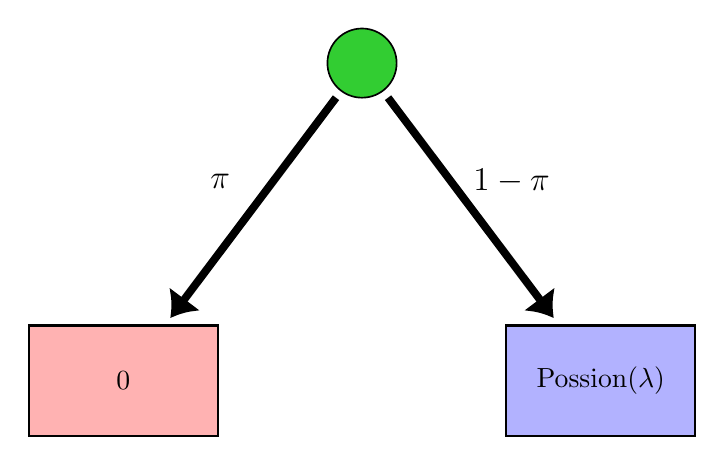
\begin{tikzpicture}[->,>=stealth',shorten >=1pt,auto,node distance=3.5cm,semithick]
                    
\node[state, fill = LimeGreen](X0){};
\node[redbox] (X1)[below left =  3cm and 1.5cm of X0]{\centerline{0}};
\node[bluebox](X2)[below right = 3cm and 1.5cm of X0]{\centerline{Possion($\lambda$)}};
 
\draw[-{Latex[length=3mm,width=5mm]}, line width=1mm, shorten <= 1mm, shorten >= 1mm] (X0)--(X1);
\draw[-{Latex[length=3mm,width=5mm]}, line width=1mm, shorten <= 1mm, shorten >= 1mm] (X0)--(X2);

\node (XX)  at (-1.8,-1.5) {\large $\pi$};
\node (XX)  at (+1.9,-1.5) {\large $1-\pi$};

\end{tikzpicture}
\end{center}

\end{document}

